%!TEX program = xelatex
\documentclass[10pt, compress]{beamer}
\usetheme[titleprogressbar]{m}

\usepackage{booktabs}
\usepackage[scale=2]{ccicons}
\usepackage{minted}
\usepackage[absolute,overlay]{textpos}
\usepackage{graphicx}


\usepgfplotslibrary{dateplot}

\usemintedstyle{trac}

\title{The Effect of Electronic Health Records Adoption
on Patient-specific Health Education Prescription, Time Utilization, and Returned Appointments: A Propensity Score Weighted Analysis}
\subtitle{}
\date{April 10, 2015}
\author{Huade Huo}
\institute{Georgetown University}

\begin{document}

\maketitle
\section{Introduction}
\begin{frame}{Background}

     
      \begin{itemize}
        \item The United States spent 17.9\% of GDP on health expenditure in 2012 
        \item Medicare and Medicaid provide financial incentive for the adoption and use of the EHR system. 
        \item ``more than half of eligible providers have qualified for and received incentive payments for adoption of certified electronic health records.'' -- The White House
      \end{itemize}

\end{frame}

\begin{frame}{Research question}

     
Will the adoption of Electronic Health Records system affect
patient-specific health education prescription, time utilization, and returned appointments?

\end{frame}

\section{Literature review}
\begin{frame}{Industril background}

     
      \begin{itemize}
        \item In 2009, the US Congress passed the American Recovery and Reinvestment Act (ARRA), which appropriates funds to promote the adoption and use of health information technology (HIT). 
        \item In order to receive the EHR stimulus money, the HITECH act (ARRA) requires eligible physicians to show ``meaningful use'' of an EHR system. 
        \item In order to demonstrate meaningful use in 2014 Stage 1, eligible professionals must meet 13 required core objectives and 5 menu objectives from a list of 9.
      \end{itemize}

\end{frame}


\begin{frame}{Prior researches}

     
      \begin{itemize}
        \item Mixed effect on health expenditure 
        \item Very limited literature evaluated the effect of EHR on the utilization of patient-specific education resources. 
        \item The effect of EHR system adoption on time efficiency is mixed and varies among different institutions.
        \item Evaluations of the effect of EHR on patient follow-up rates are limited.
        \item On the micro level, EHR has a mixed effect on cost-saving in physician practices.
      \end{itemize}

\end{frame}

\begin{frame}{Contributions}

     
This paper contributes to the literature with a national-level perspective, empirically evaluating the outcome of EHR adoption on patient-specific health education prescription rates, patient interaction time, and returned appointment rates. 


\end{frame}

\section{Analysis Plan}


\begin{frame}{Analysis Plan}

     
      \begin{enumerate}
        \item Data 
        \item Estimating treatment effect with observational data 
        \item Assumption of causal inference
        \item Propensity score estimation
        \item Propensity score weighted regression model
        \item Sensitivity tests
      \end{enumerate}
\end{frame}

\begin{frame}{Data}

National Ambulatory Medical Care Survey (NAMCS) public use micro-data files:   
      \begin{itemize}
        \item  National probability sample survey of visits to office-based physicians. 
        \item NAMCS data can be used to make physician estimates as well as visit estimates.
        \item NAMCS has information includes whether the physician practice has EHR system.
      \end{itemize}

\end{frame}

\begin{frame}{Estimating treatment effect with observational data}
   
      \begin{itemize}
        \item  Ideally, we would observe a physician in three possible conditions: one in which she has fully adopted the EHR system, one in which she has partially adopted the EHR system, and one in which she has not. 
        \item However, people in "treatment 1", "treatment 2", and "control" groups likely different in both observed and unobserved ways.
      \end{itemize}

\end{frame}

\begin{frame}{Assumption of causal inference}
   Assumptions in causal analysis:
      \begin{itemize}
        \item  Stable unit treatment value assumption (SUTVA)
        \item  Unconfoundedness assumption.
      \end{itemize}
	To estimate the effect of EHR adoption on physician behavior, we can obtain the following model:

\begin{equation*}
Y_{i} = \beta_0 + \beta_1 W_i + \Sigma^k_{i=2} \beta_k X_{ik} + \epsilon_{i}
\end{equation*}

\end{frame}

\begin{frame}{Propensity score estimation}
      \begin{itemize}
        \item  Propensity score methods attempt to replicate two features of randomized experiments.
        \begin{itemize}
			\item Propensity score methodologies can create groups that look only randomly different from one another (at least on observed variables). 
            \item Propensity score methods do not use outcome variables when setting up the design.
		\end{itemize}
        \item  Generalized Boosted Machine models (GBM) outperform simple logistic regression models in terms of bias reduction and mean squared error.
        \item We can check balance statistics after propensity score weighting (or matching).
      \end{itemize}

\end{frame}

\begin{frame}{Propensity score weighted regression model}
Let  $p_W(\mathbf{X}_i)$ denotes propensity score for physician $i$ with treatment $W$, the weights satisfy

\begin{equation*}
\omega_i[t]=\frac{1}{p_W(\mathbf{X}_i)}
\end{equation*} 

Propensity score weighting has two advantages.
      \begin{itemize}
        \item Propensity score weighting permits most types of multivariate outcome analysis and does not require an outcome variable that is continuous or normally distributed. 
        \item Unlike matching techniques, the weighting method maintains sample size.
      \end{itemize}

\end{frame}

\begin{frame}{Sensitivity tests}

      \begin{itemize}
        \item First, we tested the robustness of the result with different covariate controls in multinomial propensity score weighted regression models.
        \item Second, we examined whether the results are robust to different multinomial propensity score weighted generalized regression models.
        \item Third, we checked whether the results are robust to propensity score weighted binary treatment assignments.
        \item Fourth, we tested the robustness of the result with a propensity score matching approach.
      \end{itemize}

\end{frame}

\section{Descriptive Statistics}

\begin{frame}{Nominal and ordinal variables}

      \begin{itemize}
        \item The adoption rate of the EHR system is grew rapidly after the implementation of the EHR incentive program.
        \item Health Maintenance Organizations (80.51\%) are the most likely to fully adopt the EHR system among all health care practice owners.
        \item The full adoption rate of MSA areas (32.93\%) and non-MSA areas (33.08\%) is close to the national average (32.94\%)
        \item In general, practices with higher numbers of managed care contracts tend to have higher adoption rates of the EHR system.
        \item Among all physician specialties, general and family practices are the most likely to fully adopt the EHR system. Ophthalmologists are least likely to adopt the EHR system.
      \end{itemize}
      \end{frame}
      
\begin{frame}{Continuous variables}

      \begin{itemize}
        \item The adoption status of the EHR system has potential influence on outcome variables.
        \item There is no significant age difference between the fully treated group and the control group.
        \item Fewer patients patient with complex chronological conditions visited practices without an EHR system.
        \item Practices with full EHR adoption tended to have a higher percentage of privately insured patients.
      \end{itemize}
      \end{frame}
      
\section{Propensity score balance}

\begin{frame}{Measuring propensity score balance (1)}

The goal of propensity score weighting is to have similar covariate distribution (or ``balance'') in the weighted treated and control groups. 

We relied on the absolute standardized mean difference (ASMD, also referred to as the absolute standardized bias or the effect size) to assess the balance. 


\end{frame}

\begin{frame}{Measuring propensity score balance (2)}
The ASMD $d_x$ was calculated as the absolute difference in means between two different groups, divided by the square root of the average sample variances for these two groups

\begin{equation*}
d_x =\frac{|\Delta M_x|}{S_x}
\end{equation*}

where $\Delta M_x$ is the difference of means between two groups. $S_x$ is calculated by: 

\begin{equation*}
S_x=\sqrt{\frac{S^2_{xt}+S^2_{xp}}{2}}
\end{equation*}

where $S^2_{xt}$ and $S^2_{xp}$ denote the standard deviations of variable $x$ in group $t$ and group $p$.

\end{frame}

\begin{frame}{Sufficient iterations of GBM model}

\begin{figure}
\centering

   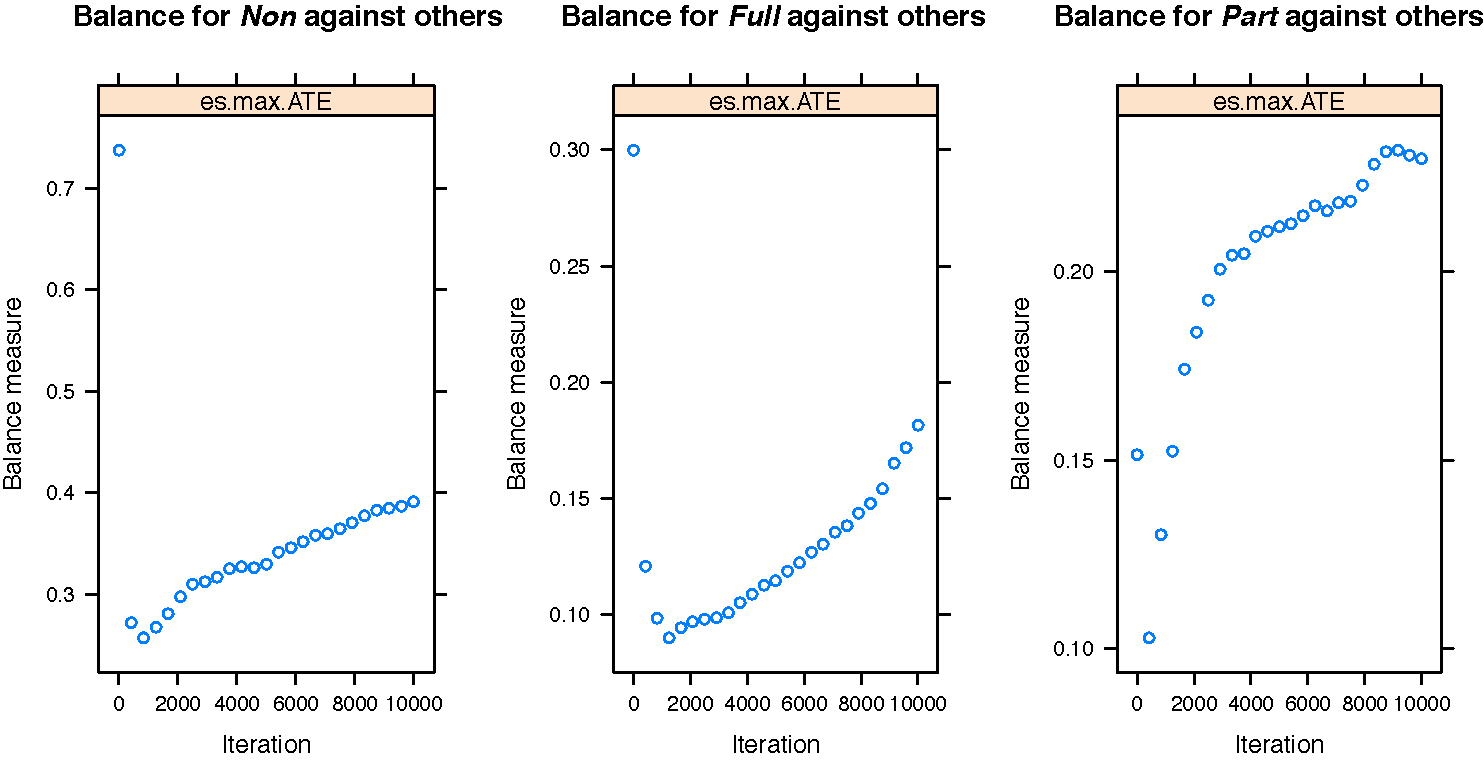
\includegraphics[width= 0.85\textwidth]{psdiag1.pdf}

\end{figure}
\end{frame}

\begin{frame}{Overlapping assumption satisfied}

\begin{figure}
\centering

   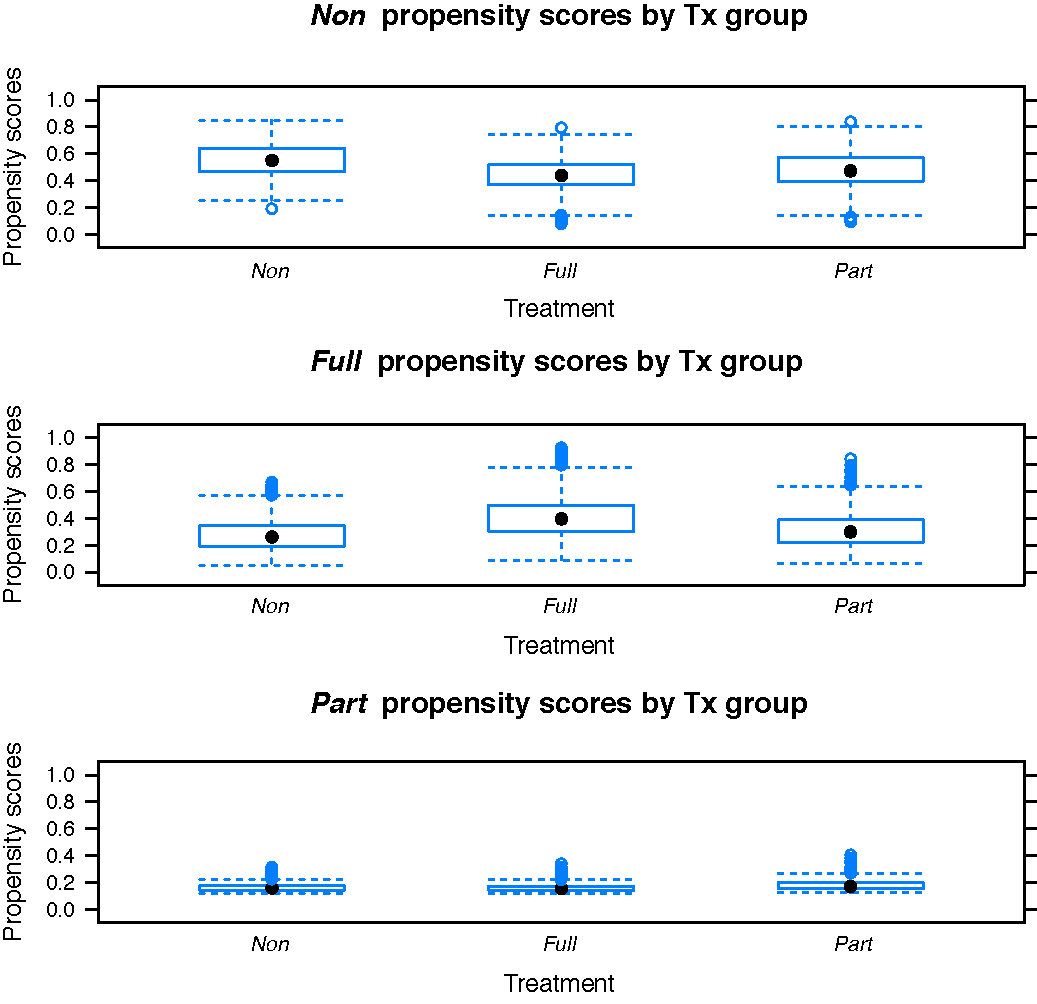
\includegraphics[width= 0.65\textwidth]{psdiag2.pdf}

\end{figure}
\end{frame}

\begin{frame}{Propensity score balance achieved (overall)}

\begin{figure}
\centering

   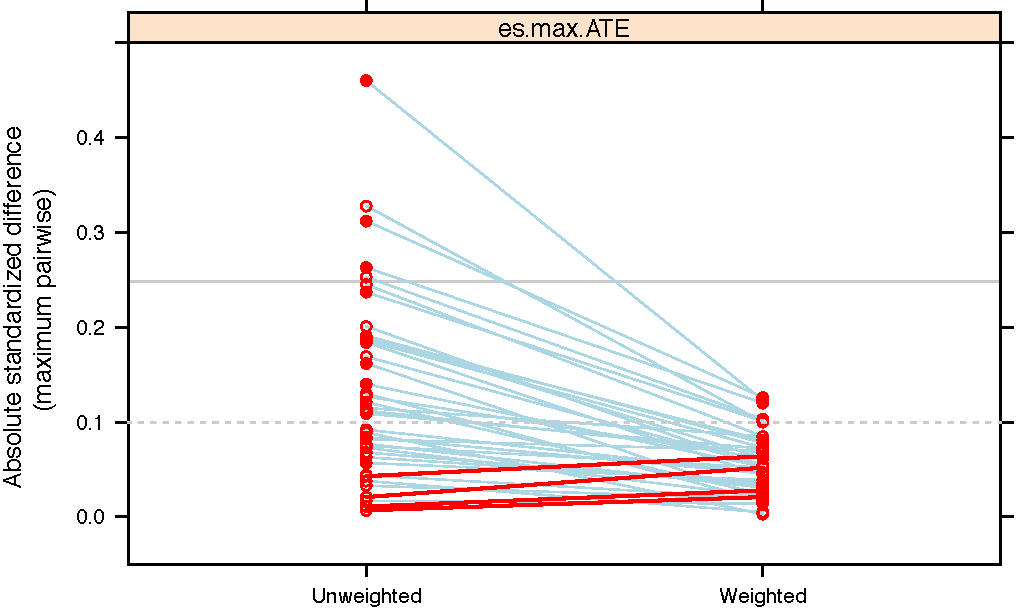
\includegraphics[width= 0.85\textwidth]{psdiag3.pdf}

\end{figure}
\end{frame}

\begin{frame}{Propensity score balance achieved (by treatments)}

\begin{figure}
\centering

   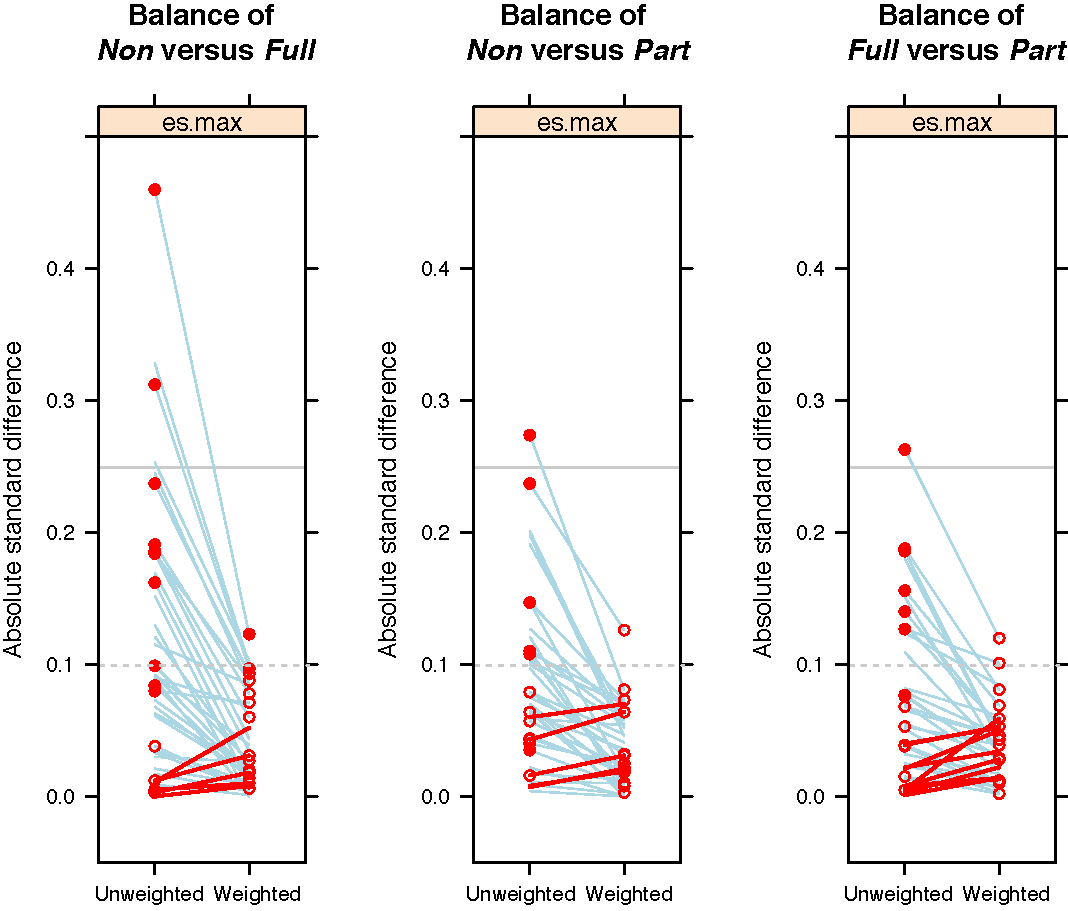
\includegraphics[width= 0.75\textwidth]{psdiag4.pdf}

\end{figure}
\end{frame}

\section{Regression results}

\begin{frame}{Patient-specific health education prescription rates}

\begin{figure}
\centering
\begin{textblock*}{8.5cm}(0.5cm,-2.5cm)
   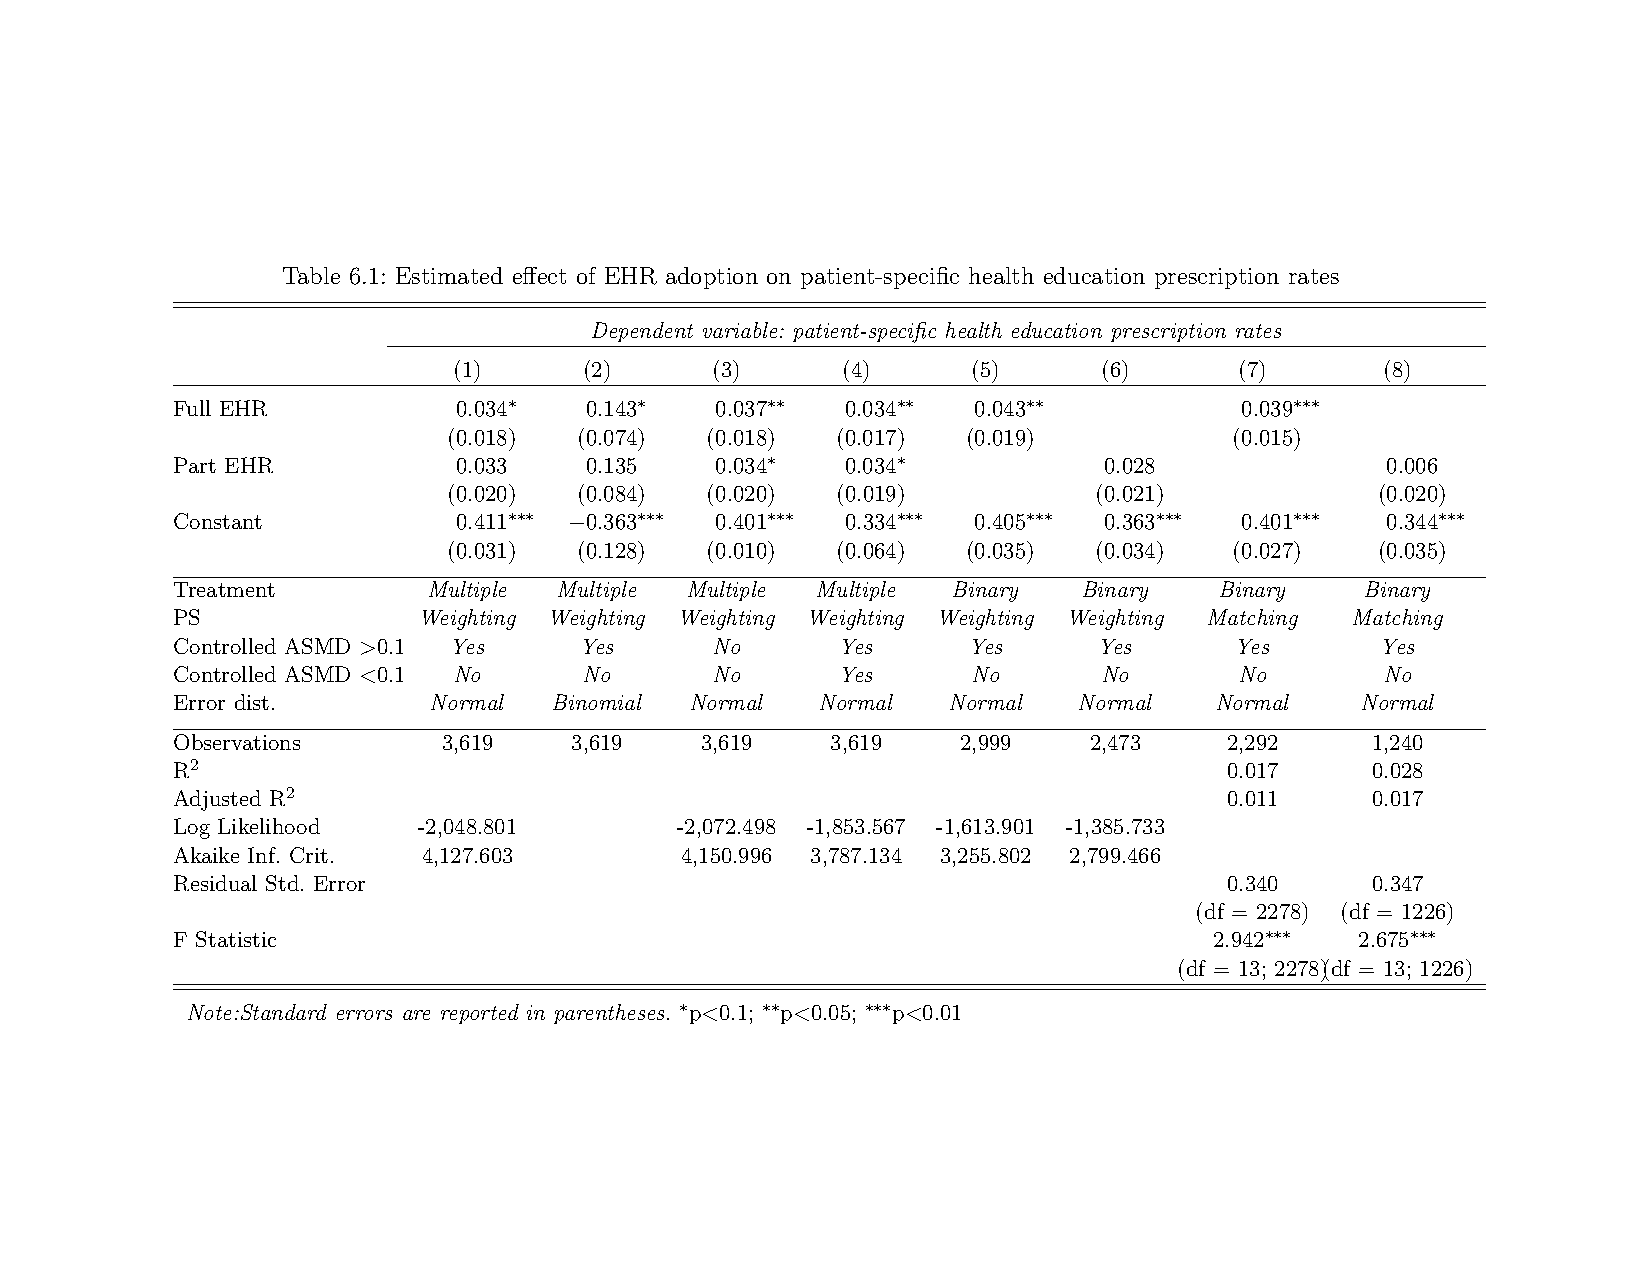
\includegraphics[width= 0.85\textwidth]{61.pdf}
\end{textblock*}
\end{figure}


\end{frame}

\begin{frame}{Time utilization}

\begin{figure}
\centering
\begin{textblock*}{8.5cm}(0.5cm,-2.5cm)
   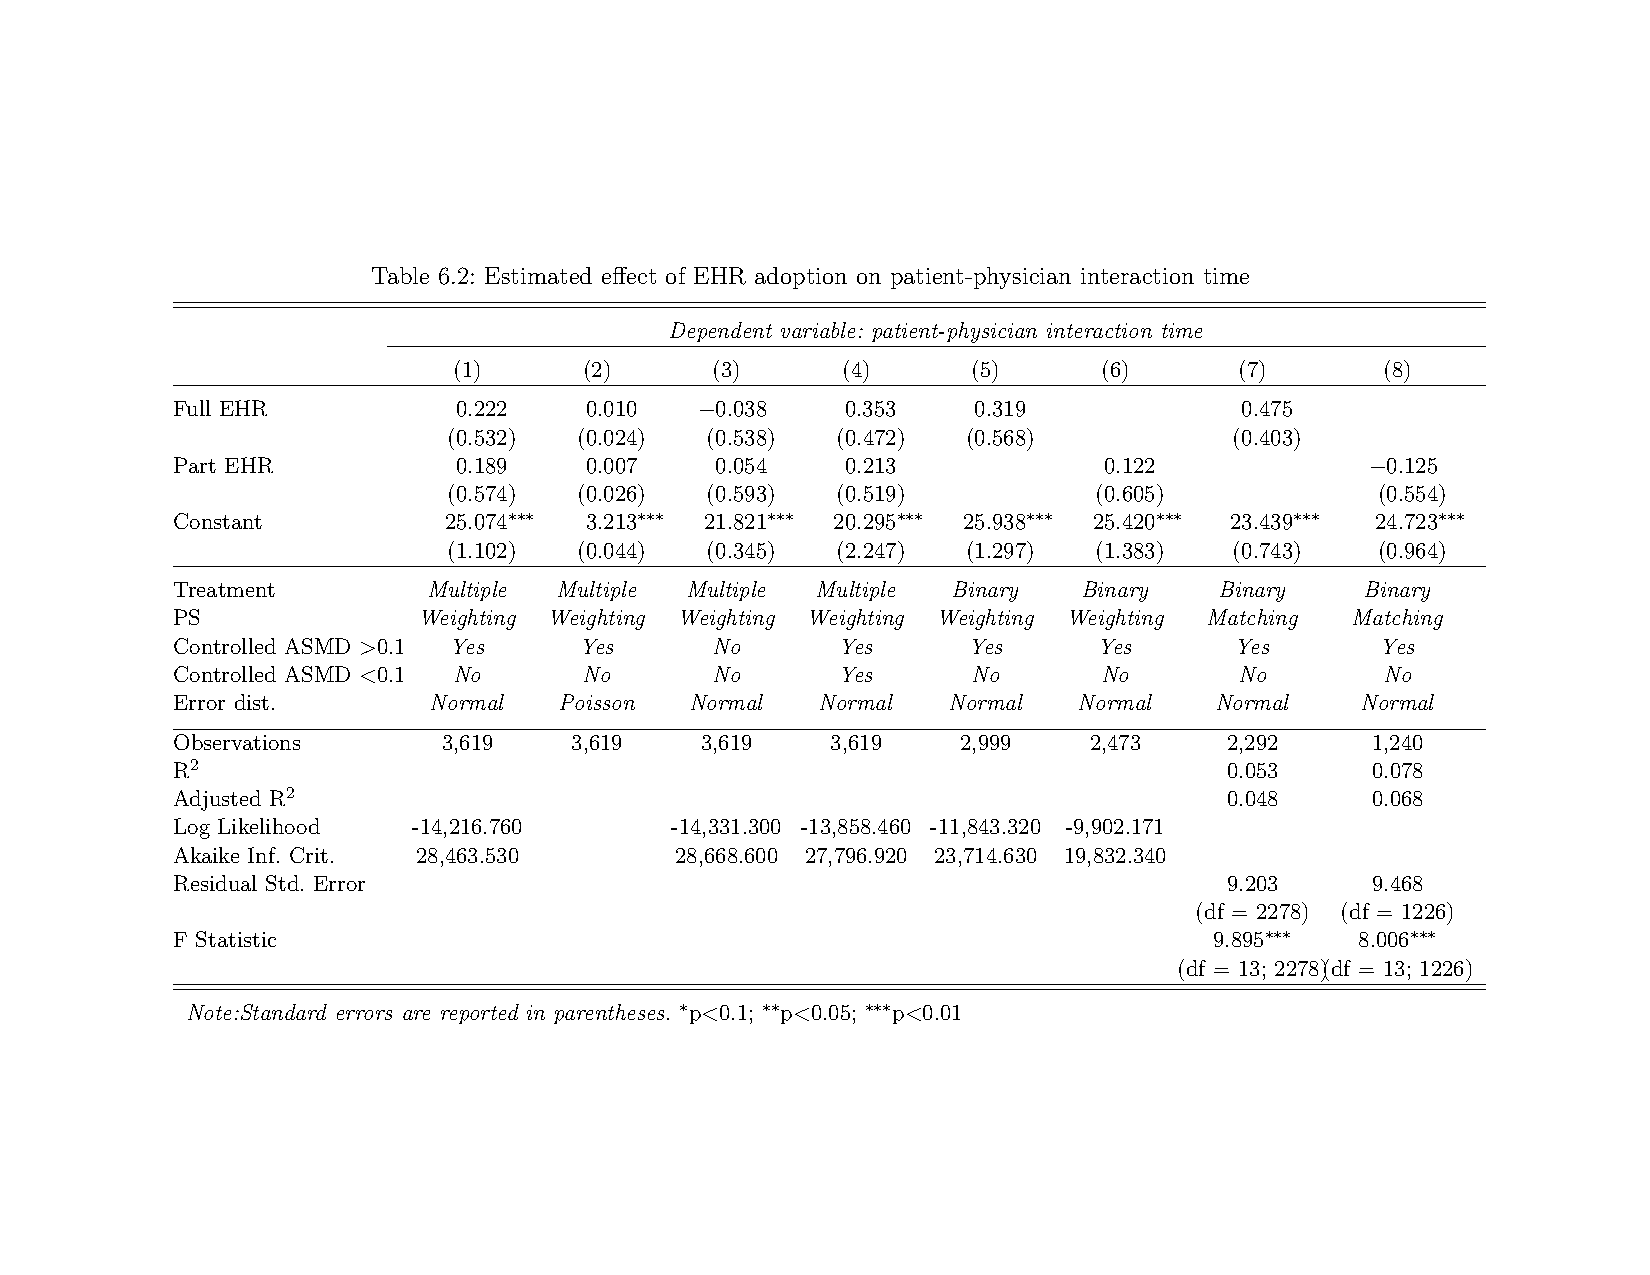
\includegraphics[width= 0.85\textwidth]{62.pdf}
\end{textblock*}
\end{figure}


\end{frame}

\begin{frame}{Returned appointment rates}

\begin{figure}
\centering
\begin{textblock*}{8.5cm}(0.5cm,-2.5cm)
   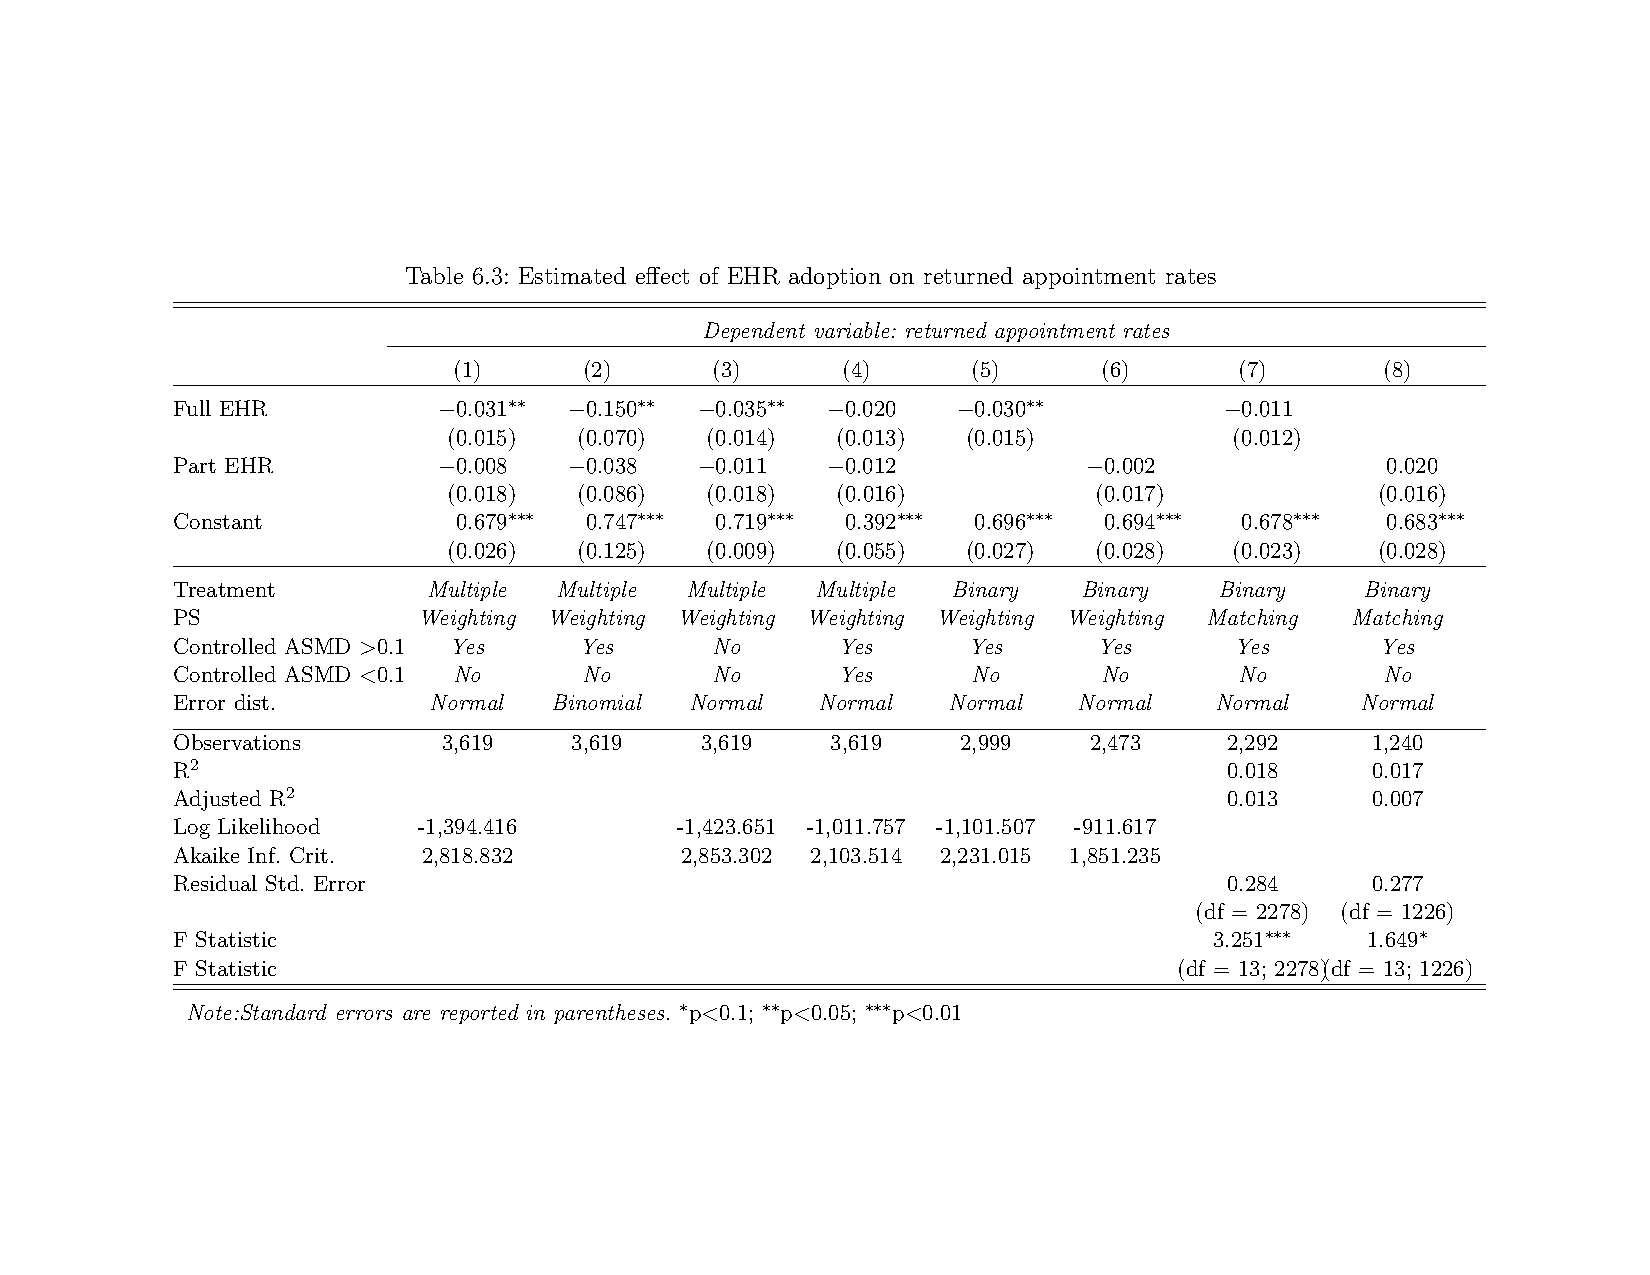
\includegraphics[width= 0.85\textwidth]{63.pdf}
\end{textblock*}
\end{figure}


\end{frame}

\section{Discussion}

\begin{frame}{Patient-specific health education prescription rates}

     There are multiple plausible reasons that can explain the EHR's positive effect on patient-specific health education prescription rates.
      \begin{itemize}
        \item First, patient-specific education resources are easy to prescribe with the EHR system. 
        \item Second, the EHR incentive program has set patient-specific education as a menu objective. 
        \item Third, physicians may intentionally use the EHR for shared decision-making and education to improve patient engagement. 

      \end{itemize}

\end{frame}

\begin{frame}{Time utilization}

     Several factors contributed to a mixed-time utilization outcome after EHR adoption.
      \begin{itemize}
        \item On the one hand, time efficiency could have improved as physicians became familiar with EHR systems. 
        \item On the other hand, certain EHR systems have poor usability. 
        \item Additionally, physicians could have continued to perform certain tasks using paper-based methods, even though the computer automatically performed these tasks for them.

      \end{itemize}

\end{frame}


\begin{frame}{Returned appointment rates}

     EHR adoption has a negative (although not robust) effect on returned appointment rates. There are a few hypothetical explanations.
      \begin{itemize}
        \item First, the EHR system may improve the quality of treatment, and thus, there would be no need to revisit the physician. 
        \item Second, the patient may disregard the automatic reminder generated by the EHR system. 
        \item Third is alert fatigue experienced by physicians; they routinely ignore alerts due to the high volume generated by the EHR system. 
      \end{itemize}

\end{frame}


\begin{frame}{Limitations}

     
      \begin{itemize}
        \item A specific patient who has multiple encounters at the survey site in a certain year has a heavier weight than a counterfactual patient who used health care less frequently. 
        \item Our casual inference method is based on strong assumptions due to the limitation of observational data. 
        \item The effect of EHR system adoption on time efficiency is mixed and varies among different institutions.
        \item Evaluations of the effect of EHR on patient follow-up rates are limited.
        \item Empirical research on the casual relationship between studied outcomes and health quality is still limited.
      \end{itemize}

\end{frame}

\begin{frame}{Policy implications}

     
      \begin{itemize}
        \item The first is linking patient education with quality improvement efforts.
        \item Second, the CMS should work with physicians and vendors to improve the usability of EHR systems. 
      \end{itemize}

\end{frame}

\plain{Questions?}

\end{document}